
\section{Tasks}
\label{cp6:tasks}



\subsection{Tasks}
\label{sec:experiment-tasks}



We expect the experiment to be executed offline, i.e., the experiment has self-contained instructions that allow a participant to perform their assigned tasks without any supervision.
\gm{Why not just say the participants
completed the tasks on their own time?}
This requires tasks that are easy to understand and perform in a single experimental session. At the same time, our main hypothesis requires tasks for which a developer will likely benefit from the use of additional information to complete.


These criteria lead us to select Python w3resource tasks\footnote{\url{https://www.w3resource.com/python-exercises/}}
that required usage of at least one module external to the Python core modules~\cite{thiselton2019}.
By using an external module, we aim to reduce the likelihood that a participant 
can provide a solution for a task without consulting any of the artifacts accompanying that task. 






Table~\ref{tbl:python-tasks-modules} details the tasks that we have selected. 
We chose these tasks due to how they focus on modules widely adopted both by open source systems and by private companies.
For example, the \texttt{NYTimes} task involves using a HTML parser, namely \texttt{BeautifulSoup},
which Reddit---a social news aggregator with approximately 430 million monthly users---uses 
to parse urls and identify images shown on its posts' headlines~\cite{bs4-reddit}. 
Similarly, the \texttt{Titanic} task encompasses using \texttt{Pandas}, a data analysis and manipulation module
used in many open source data science projects~\cite{ma2017, shrestha2020}.





\begin{table}
\centering
\caption{Python tasks}
\begin{footnotesize}
\rowcolors{2}{}{lightgray}
\begin{tabular}{ll}
\hline
\textbf{Task} & \textbf{Description}                                                                                         \\
\hline
\hline
%
\parbox[l][1cm][c]{1cm}{Practice task}       &
\parbox[l][1cm][c]{11cm}{Given three dictionaries representing address books,
you must write an algorithm using the Python core \texttt{dict} module to merge them.}    \\
\hline
%
Distances     &
\parbox[l][1.3cm][c]{11cm}{Given a string representing a rendezvou point and a list of suggested picnic addresses
    you must write an algorithm using the \texttt{geopy} module to find the  picnic address closest to the rendezvou point.} \\
%
NYTimes       &
\parbox[l][1cm][c]{11cm}{Given a string representing the url for NY Times Today's,
    write an algorithm using the \texttt{BeautifulSoup} and \texttt{requests} modules to scrape all the headlines of that page.}
\\
%
Titanic       &
\parbox[l][1cm][c]{11cm}{Given a string representing a url for the titanic dataset,
    you must write an algorithm using the \texttt{pandas} and \texttt{seaborn} modules to create a barchart of the data.}    \\
    
\hline
\end{tabular}
\end{footnotesize}
% \smallskip
\label{tbl:python-tasks-modules}
\end{table}









\subsection{Artifacts}
\label{sec:experiment-artifacts}


Each task requires a set of artifacts that a participant could peruse for information that could assist them complete the task.
We select artifacts for a task following procedures similar to the ones we used to create the \acs{DS-android} dataset (Chapter~\ref{ch:android-corpus}). 
For each of the tasks in Table~\ref{tbl:python-tasks-modules}, we use the Google search engine to obtain up to ten artifacts that likely contain relevant
information for that task. 





\subsection{Colab}
\label{cp6:environment}


To ensure that participants had the same conditions to perform each task
and also to minimize setup instructions, we used Google Colab\footnote{\url{https://colab.research.google.com/}} as our coding environment. 
% By using Colab, we also expect setup instructions to be minimal 
% so that we allow a participant to focus on the task and experimental procedures.



Figure~\ref{fig:nytimes-task-colab} shows an example of our online environment for the \texttt{NYTimes} task.
At the left-hand side, participants had the task description and examples of input and output scenarios as well as a list of resources associated with that task. 
By clicking on the coding environment link, participants were redirected to Colab (right-hand side),
where they had a code editor with amenities commonly found in modern IDEs, such as code completion and syntax highlighting. 



Through Colab, a participant could compile their solution and test it against the examples shown alongside the task description.
Upon testing, the system would display full details about the test cases, e.g., the test's input, which assertion failed, and why. 




\clearpage

\begin{landscape}
\begin{figure}
    \centering
    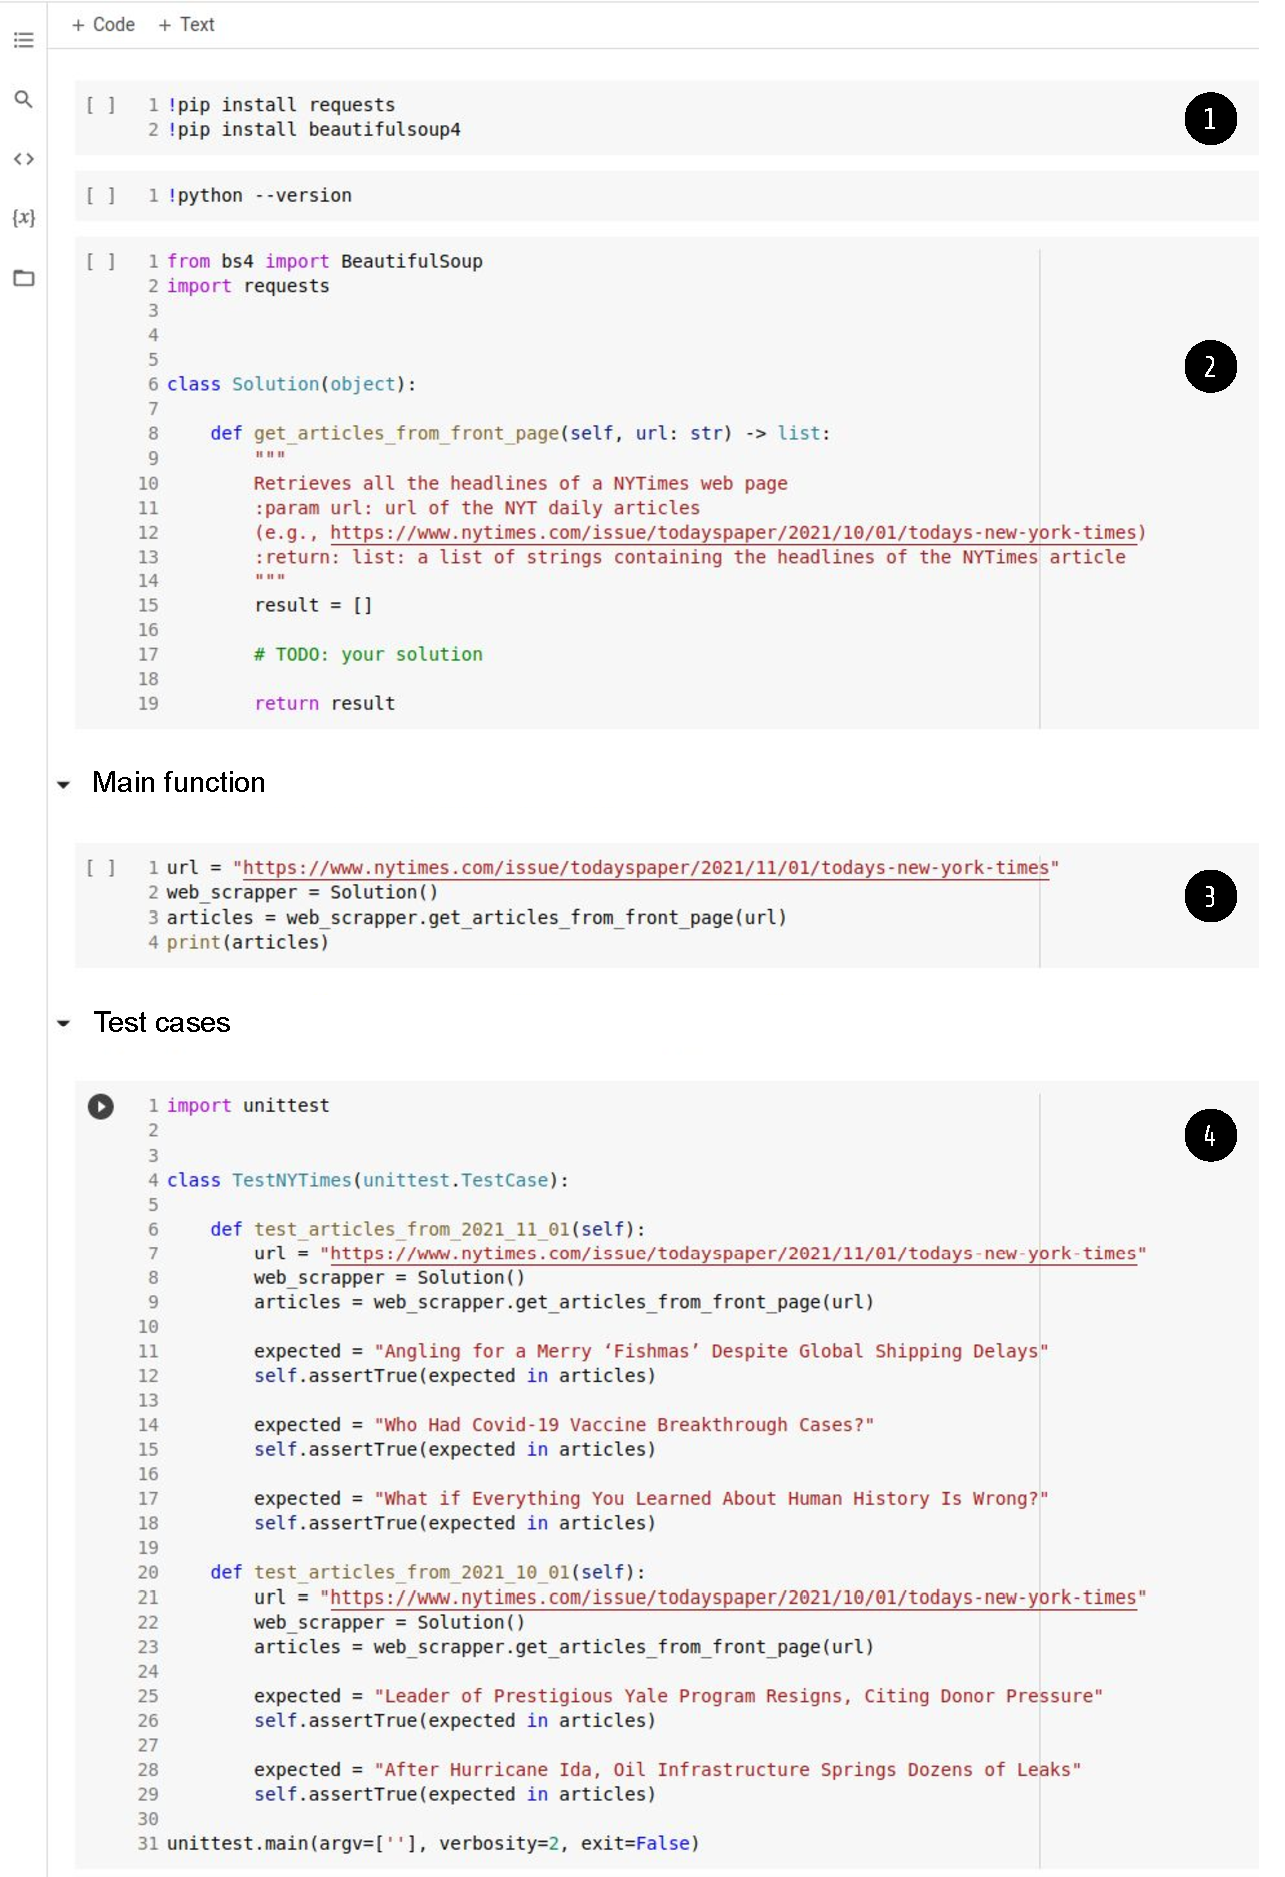
\includegraphics[width=1.5\textwidth]{cp6/task-colab.pdf}
    \caption{NYTimes task and Colab environment.}
    \label{fig:nytimes-task-colab}
\end{figure}
\end{landscape}
